\documentclass[a4paper,12pt]{article}

% Pacchetti essenziali
\usepackage[utf8]{inputenc}
\usepackage[T1]{fontenc}
\usepackage[italian]{babel}
\usepackage{geometry}
\geometry{top=2.5cm, bottom=2.5cm, left=2.5cm, right=2.5cm}
\usepackage{hyperref}
\hypersetup{
	colorlinks=true,
	linkcolor=blue,
	urlcolor=blue,
	pdftitle={Manuale Utente - Portale Cori San Vito},
	pdfsubject={Manuale utente}
}
\usepackage{graphicx}
\usepackage{enumitem}
\usepackage{booktabs}
\usepackage{array}
\usepackage{xcolor}

% Comandi personalizzati
\newcommand{\roleadmin}{\texttt{admin}}
\newcommand{\roledirettore}{\texttt{direttore}}
\newcommand{\roleresponsabile}{\texttt{responsabile}}
\newcommand{\rolecorista}{\texttt{corista}}
\newcommand{\rolestrumentista}{\texttt{strumentista}}

\setlist[itemize]{topsep=5pt, itemsep=0pt}

\usepackage{titlesec}
\titleformat{\subsubsection}{\normalfont\fontsize{13}{15}\selectfont\bfseries}{\thesubsubsection}{1em}{}

\begin{document}
	
	\begin{titlepage}
		\centering
		{\Huge\bfseries Manuale per l'utente \par}
		\vspace{0.5cm}
		{\Large Portale dei Cori San Vito\par}
		\vspace{1cm}
		{\large Versione 1.0 -- \today\par}
		\vspace{1.5cm}
		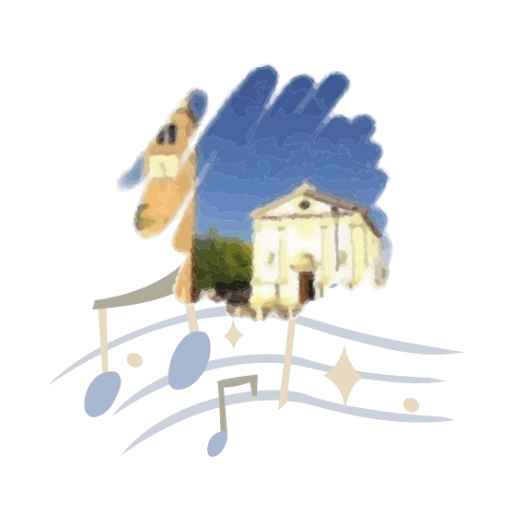
\includegraphics[width=0.5\textwidth]{../images/web-app-manifest-512x512.png} % se disponibile
		\vfill
		{\large Parrocchia di San Vito e C.M. -- Spinea (VE)\par}
		\vspace{0.3cm}
		{\large Sviluppato e mantenuto da Anna Ficotto\par}
		\vspace{0.3cm}
		{\large \textit{\href{https://corisanvito.github.io}{corisanvito.github.io}}\par}
	\end{titlepage}
	
	{\hypersetup{linkcolor=black}
		\tableofcontents}
	\newpage
	
	\section{Introduzione}
	Il portale \textbf{Cori San Vito} è il sito web ufficiale dei cori che animano la Santa Messa domenicale delle ore 10 e delle 11:15 della parrocchia di San Vito e C.M. a Spinea (VE).  
	Lo scopo del progetto è quello di riunire tre cori (\textit{Coro delle 10}, \textit{Coro delle 11:15} e \textit{Coro Estivo}) in un unico portale, mettendo a disposizione di tutti i coristi, dei musicisti e dei responsabili gli strumenti necessari per la gestione quotidiana e settimanale del gruppo.
	
	Il portale è composto da due aree principali:
	\begin{itemize}
		\item \textbf{Area pubblica} (accessibile a tutti): home page di selezione del coro, repertorio canti con ricerca, pagine di dettaglio per ogni coro.
		\item \textbf{Area riservata} (\texttt{/portale}): accessibile solo dopo il login, con funzionalità differenziate in base al ruolo.
	\end{itemize}
	
	
	\section{Visione e spirito del progetto}
	Il portale nasce da un'esigenza concreta, ma si radica in qualcosa di più profondo: la convinzione che il canto liturgico sia un atto di servizio -- verso la comunità, verso la celebrazione e verso Dio.
	
	I cori della parrocchia di San Vito non sono gruppi di esecutori: sono parte viva dell'assemblea, e il loro compito è quello di \textit{guidare} e \textit{sostenere} la preghiera cantata di tutti i fedeli. È con questo spirito che è nato questo strumento: non per complicare, ma per \textbf{semplificare il lavoro quotidiano} di chi ogni settimana si mette a disposizione.
	
	Il progetto è "artigianale", fatto con cura e pensato su misura per chi lo usa. Non è un prodotto commerciale, ma il frutto di un lavoro condiviso: la parte informatica è curata da chi scrive, ma i contenuti, le idee e il senso del tutto vengono dalle persone che animano questi cori ogni domenica.
	
	L'obiettivo finale è uno solo: che il canto dell'assemblea sia sempre più bello, più partecipato e più consapevole. Tutto il resto -- i repertori, le presenze, la bacheca, gli spartiti -- è al servizio di questo.
	
	
	\section{Come si accede al portale}
	
	L'accesso all'area riservata avviene tramite la pagina \texttt{/portale/login}.  
	Per effettuare il login è necessario disporre di un account e del token di autenticazione fornito dai responsabili (password).
	
	
	\section{Area pubblica (senza login)}
	
	\subsection{Home page di selezione coro}
	
	La home page principale permette di scegliere il coro di interesse. Ogni coro ha una propria pagina dedicata con una palette colori specifica. In questa pagina si trovano i canti della prossima celebrazione liturgica animata dal coro, i canti da imparare o ripassare e, quando disponibili, i canti dedicati a un tempo forte in particolare (ad esempio, i canti del tempo di Avvento).
	
	\subsection{Repertorio canti (\texttt{/canti})}
	
	Il repertorio è unificato per tutti i cori e include:
	
	\begin{itemize}
		\item \textbf{Ricerca full-text} su titoli, testi e categorie.
		\item \textbf{Bonus di punteggio} per corrispondenze esatte, per dare priorità ai titoli completi.
		\item \textbf{Filtraggio per categoria liturgica}.
		\item \textbf{Modalità presentazione} con scrolling automatico, utile per la proiezione durante le prove e le celebrazioni.
	\end{itemize}
	
	
	\section{Ruoli e permessi}
	
	Il portale prevede tre macro-livelli di accesso, come riassunto nella tabella seguente:
	
	\begin{table}[h]
		\centering
		\begin{tabular}{>{\bfseries}l p{10cm}}
			\toprule
			Ruolo & Permessi \\
			\midrule
			\roleadmin & Accesso completo a \textbf{tutti} i cori e a tutte le funzioni (supervisione totale). L'unico amministratore del sito è Anna Ficotto, in quanto sviluppatrice.\\
			\roledirettore \space / \roleresponsabile & Gestione completa del \textbf{proprio coro} di appartenenza: bacheca, gestione dei canti e della home page del coro, possibilità di aggiungere nuovi canti, possibilità di correggere un canto, calendario, gestione degli utenti, registro delle presenze e statistiche, scambio di spartiti/accordi con i musicisti, profilo personale. Le funzioni sono identiche per entrambi i ruoli. \\
			\rolecorista & Area personale: bacheca, calendario, possibilità di suggerire una correzione, profilo personale.\\
			\rolestrumentista & Area personale: bacheca, calendario, possibilità di suggerire una correzione, possibilità di scambio di spartiti/accordi con gli altri musicisti, profilo personale.\\
			\bottomrule
		\end{tabular}
		\caption{Ruoli e permessi del portale}
		\label{tab:ruoli}
	\end{table}
	
	
	
	
	\section{Area riservata (\texttt{/portale})}
	Dopo il login, l'utente accede alla \textbf{dashboard} (\texttt{/portale/}), dove vengono mostrate le card dinamiche in base al ruolo.
	
	\subsection{Funzioni per tutte le categorie di utente}
	\subsubsection{Bacheca avvisi (\texttt{/portale/bacheca})}
	La bacheca mostra gli avvisi, filtrati per:
	\begin{itemize}
		\item \textbf{generali} (visibili a tutti)
		\item \textbf{specifici per coro} (visibili solo ai membri di quel/quei coro/i)
		\item \textbf{personali} (indirizzati ad alcuni utenti specifici)
	\end{itemize}
	
	\subsubsection{Calendario (\texttt{/portale/calendario})}
	Il calendario integrato con Google Calendar mostra prove, celebrazioni e altri eventi specifici  coro per coro.\\
	
	\textbf{Per direttori e responsabili}: per poter modificare il calendario, è necessario che esso sia condiviso con la vostra mail personale. Per eventuali problemi contattare l'amministratore.
	
	\subsubsection{Correggi un canto (\texttt{/portale/correggi-canto})}
	La pagina dà la possibilità ad ogni membro del gruppo di inviare una segnalazione di errore per un canto specifico.\\
	Colgo l'occasione per ricordare che questo servizio è in continuo aggiornamento, ed è frutto sì del lavoro di sviluppo informatico della sottoscritta, ma anche e soprattutto dello spirito di gruppo e di servizio dei cori che lo utilizzano. È proprio per questo motivo che si decide di inserire questa sezione: per dare spazio a correzioni e segnalazioni che, si sottolinea, sono utili a tutti gli utenti di questo servizio.
	
	\subsubsection{Spartiti e accordi (\texttt{/portale/spartiti})}
	Questa sezione, dedicata solo ai musicisti, è, di fatto, un archivio di materiali come spartiti, accordi e altri documenti "musicali", che ognuno ha la possibilità di visualizzare e caricare.\\
	Per caricare un file bisogna:
	\begin{itemize}
		\item \textbf{scegliere un canto} dal menu a discesa;
		\item \textbf{inserire la tonalità};
		\item \textbf{indicare gli strumenti} a cui quel materiale è riferito;
		\item \textbf{allegare i file}, per un massimo di 5 di qualsiasi formato (si suggerisce di preferire i file PDF alle immagini, perché più nitidi e facili da stampare).
	\end{itemize}
	
	Nel caso si inserissero più materiali per lo stesso canto, questi verranno raggruppati in una stessa sezione, dove si possono trovare con facilità. Per questo motivo, non preoccupatevi di dover inserire tutto con un solo caricamento!
	
	\subsubsection{Profilo personale (\texttt{/portale/profilo})}
	Tutti gli utenti possono:
	\begin{itemize}
		\item visualizzare e modificare i propri dati personali
		\item indicare il proprio \textbf{timbro  vocale e/o strumento musicale}
		\item cambiare la password
	\end{itemize}
	Per modificare le altre informazioni, in particolare i cori in cui si presta servizio, è necessario contattare il proprio responsabile e/o direttore e obbligatoriamente anche l'amministratore del sito scrivendo una mail a \href{mailto:corisanvito@gmail.com}{corisanvito@gmail.com}.
	
	
	\subsection{Funzionalità per direttori e responsabili}
	In aggiunta alle pagine elencate sopra, vi sono delle sezioni visibili e utilizzabili esclusivamente dagli utenti con ruolo di \roleresponsabile \space oppure di \roledirettore. \\
	\textit{Nota: per \roledirettore{} e \roleresponsabile{} le funzioni sono assolutamente identiche.}
	
	\subsubsection{Bacheca avvisi (\texttt{/portale/bacheca})}
	L'unica differenza con gli altri utenti consiste nel poter anche aggiungere degli avvisi. Bisognerà inserire:
	\begin{itemize}
		\item il titolo dell'avviso;
		\item il testo del messaggio;
		\item i destinatari che, come sopra spiegato, possono essere tutti gli utenti di uno o più cori, una sezione specifica di uno o più cori (ad esempio, "tutti i contralti del Coro delle 10 e del Coro Estivo"), oppure degli utenti specifici (selezionabili attraverso nome e cognome);
		\item facoltativamente gli allegati, per un massimo di 5 file di qualsiasi tipo e dimensione, che gli utenti potranno visualizzare e scaricare. Si sconsiglia di allegare file di grandi dimensioni per facilitare il caricamento sul server degli stessi.
	\end{itemize}
	\textbf{N.B.}: i messaggi saranno visibili esclusivamente agli utenti selezionati.\\
	I messaggi portano il nome di chi l'ha inserito e la data, e \textbf{possono essere eliminati in qualsiasi momento}.
	
	\subsubsection{Gestione canti (\texttt{/portale/canti-admin})}
	Da qui è possibile:
	\begin{itemize}
		\item gestire i \textbf{canti della settimana} o, più in generale, della prossima celebrazione liturgica;
		\item gestire i \textbf{nuovi canti} (da imparare o ripassare);
		\item gestire i canti dei \textbf{tempi forti} (Avvento, Natale, Quaresima, Pasqua, eccetera).
	\end{itemize}
	
	Per inserire un canto nella sezione "Canti della domenica":
	\begin{itemize}
		\item scegliere la data della domenica (quella pre-impostata è quella prossima);
		\item scegliere il momento liturgico (ingresso, acclamazione al Vangelo, offertorio, etc.);
		\item scegliere il canto;
		\item cliccare sul bottone "+".
	\end{itemize}
	Passata quella domenica, le righe della tabella con date passate verranno eliminate e lasceranno il posto ai nuovi inserimenti.\\
	
	Per inserire il \textbf{salmo}, scegliere la data della celebrazione, scegliere poi "Salmo" dalla tendina, e per ultimo inserire il "nome" della domenica o della celebrazione liturgica (ad esempio, "XVIII domenica T.O. anno A") e il link al file audio. Per questo si consiglia di far riferimento alla  \href{https://www.istitutomusicasacratreviso.it/elenco-salmi/}{sezione dedicata nel sito dell'Istituto Diocesano di Musica Sacra di Treviso}.\\
	
	Per inserire un canto, invece, nella sezione "Nuovi canti da imparare" è sufficiente selezionare il canto dalla tendina e cliccare "+". Per eliminare un canto, come nelle altre sezioni, basterà cliccare sul bottone rosso "\texttt{X}" e il canto verrà tolto da quella sezione.\\
	
	Per inserire un canto nella sezione dei tempi forti è necessario scrivere a mano il nome del tempo liturgico (ad esempio, "Natale" o "Quaresima") e successivamente scegliere il canto dal menu a tendina come per le sezioni precedenti.
	
	\subsubsection{Aggiungi un canto nuovo (\texttt{/portale/aggiungi-canto})}
	In questa pagina è disponibile un form con cui si ha la possibilità di richiedere l'aggiunta di un canto.
	
	È richiesto l'inserimento del titolo e del testo, ma è molto gradita l'indicazione anche dell'autore e della categoria (sia il momento, sia il tempo liturgico, ad esempio "avvento, offertorio").
	
	È importante, anche se non obbligatorio, inserire il link del video della canzone su YouTube, poiché lo scopo di questo sito è proprio facilitare l'insegnamento e lo studio dei canti.
	
	Ugualmente essenziale è l'inserimento del numero del canto nel libretto "Cantiamo al Signore", poiché scopo dei nostri cori è, tra le altre cose, far partecipare l'assemblea tutta alla liturgia attraverso il canto.
	
	\subsubsection{Gestione utenti (\texttt{/portale/utenti})}
	Consente di:
	\begin{itemize}
		\item creare nuovi account;
		\item attivare/eliminare utenti;
		\item assegnare ruoli;
		\item visualizzare le informazioni dei coristi dei propri cori.
	\end{itemize}
	
	Per creare un nuovo account è necessario inserire nome, cognome, email (in alternativa un nome utente) e una password temporanea insieme al ruolo del nuovo utente (\rolecorista, \rolestrumentista, \roledirettore, \roleresponsabile), i cori di cui fa parte e il timbro di voce e/o lo strumento suonato. La data di nascita e il numero di telefono non sono necessari.
	
	\subsubsection{Presenze e statistiche (\texttt{/portale/registro} e \texttt{/portale/presenze})}
	La prima pagina permette di registrare le presenze alle prove e alle celebrazioni. La seconda, invece, fa vedere le statistiche di presenza generali e individuali per ogni utente (di qualsiasi tipo).\\
	È importante che questa funzionalità sia usata principalmente per avere dei dati oggettivi se necessari, e non per premiare o meno un corista piuttosto che un altro.
	
	
	
	
	\section{Design e accessibilità}
	Il portale è \textbf{responsive} e si adatta automaticamente a desktop, tablet e smartphone. Nel caso in cui ci fosse qualcosa da sistemare o si notassero errori o bug non si esiti a scrivere a \href{mailto:corisanvito@gmail.com}{corisanvito@gmail.com}.
	
	
	\section{Ringraziamenti}	
	Un ringraziamento speciale va a \textbf{Gianpaolo}, che per primo ha creduto in questo progetto e ha contribuito con idee e intuizioni che sono diventate funzionalità concrete del portale.
	
	In secondo luogo, però, non posso non ringraziare chi questo servizio lo usa e lo apprezza ogni domenica: tutti i coristi che hanno voglia di innovarsi ancora!\\
	
	Il progetto è sviluppato e mantenuto da \textbf{Anna Ficotto}, che ne cura anche i contenuti e il supporto tecnico.
	
	
	\section{Contatti e supporto}
	Per qualsiasi problema o richiesta di assistenza, contatta la responsabile del portale scrivendo all'indirizzo email \href{mailto:corisanvito@gmail.com}{corisanvito@gmail.com}.\\
	
	Come ho ricordato più volte in questo documento, il lavoro di squadra è essenziale per il mantenimento di questo servizio, e per questo motivo ogni segnalazione o richiesta è più che ben accetta.
	
\end{document}